\documentclass[french]{article}
\usepackage{../exercices}
\usetikzlibrary{arrows,automata, positioning}
\begin{document}

% jeremy.ledent@irif.fr
\begin{center}
    \huge{\textbf{S6- Langages et expressions rationnelles}}
\end{center}

\begin{exo}
    Soient \(A,B,C\) les langages dénotés respectivement par les regex suivants
    \((bb|aba)*, (b|aba*)\) et \((ab|abb)*\). Donner les trois mots les plus courts de
    \(A\cup B\), \(A\cup C\), \(A\cap B, A\cap C\) et \(B\cap C\)
    \boxans{
        Les mots les plus courts sont
        \begin{enumerate}
            \itt \(A\cup B\) : \(\eps,b,bb\).
            \itt \(A\cup C\) : \(\eps,ab,bb\).
            \itt \(A\cap B\) : \(\eps, bb, aba\).
            \itt \(A\cap C\) : \(\eps, ababb, ababbababb\).
            \itt \(B\cap C\) : \(\eps, abab, ababb\).
        \end{enumerate}
    }
\end{exo}

\begin{exo}
    Pour chacune des expressions rationelles suivantes, donner une description
    du langage.
    \begin{q}{1}
        \(\left(\left(1\mid0\right)0\right)^*\left(\eps\mid0\mid1\right)\)
        \boxans{Tous les mots dont les caractères d'indice pair sont des \(0\).}
    \end{q}
    \begin{q}{2}
        \(\left(1\mid01\mid001\right)^*\left(\eps\mid0\mid00\right)\)
        \boxans{Tous les mots ayant au plus deux \(0\) de suite.}
    \end{q}
    \begin{q}{3}
        \(0^*\left(10^*10^*10^*\right)^*\)
        \boxans{Tous les mots contenant un nombre de \(1\) divisible par \(3\).}
    \end{q}
\end{exo}

\begin{exo}
    Pour chacun des langages sur l'alphabet \(\{0,1\}\) suivants, écrire un regex
    les reconnaissant et construire un automate déterministe le reconnaissant.
    \begin{q}{1}
        Tous les mots de longueur paire.
        \boxans{\(\left(00\mid01\mid10\mid11\right)^*\) ou \(((0\mid 1)\{2\})^*\)
        sont des Regex valide, auquel correspondent l'automate suivant\newline
        \begin{center}
            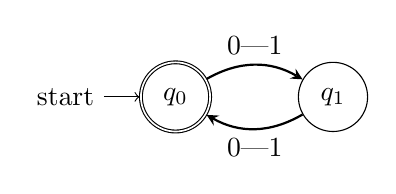
\begin{tikzpicture}[node distance = 2cm]
                \node (q0) [state,initial,accepting] {$q_0$};
                \node (q1) [state] at (2,0) {$q_1$};

                \path [-stealth, thick]
                    (q0) edge [bend left] node [above] {0|1}   (q1)
                    (q1) edge [bend left] node [below] {0|1}   (q0);
            \end{tikzpicture}
        \end{center}
        }
    \end{q}
    \begin{q}{2}
        Tous les mots contenant au moins un \(0\).
        \boxans{\(\left(0\mid1\right)^*0\left(0\mid1\right)^*\).\newline
        \begin{center}
            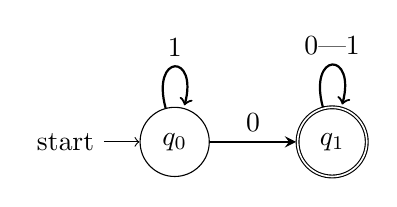
\begin{tikzpicture}[node distance = 2cm]
                \node (q0) [state,initial] {$q_0$};
                \node (q1) [state,accepting] at (2,0) {$q_1$};

                \path [-stealth, thick]
                    (q0) edge [loop above] node {1}(q0)
                    (q0) edge node [above] {0} (q1)
                    (q1) edge [loop above] node {0|1}(q1);
            \end{tikzpicture}
        \end{center}
        }
    \end{q}
    \begin{q}{3}
        Tous les mots avec un nombre impair de \(1\).
        \boxans{\(\left(0^*10^*10^*\right)10^*\).\newline
        \begin{center}
            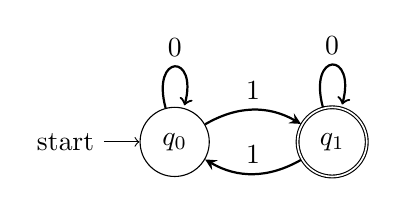
\begin{tikzpicture}[node distance = 2cm]
                \node (q0) [state,initial] {$q_0$};
                \node (q1) [state,accepting] at (2,0) {$q_1$};

                \path [-stealth, thick]
                    (q0) edge [loop above] node {0}(q0)
                    (q0) edge [bend left] node [above] {1} (q1)
                    (q1) edge [bend left] node [above] {1} (q0)
                    (q1) edge [loop above] node {0}(q1);
            \end{tikzpicture}
        \end{center}}
    \end{q}
    \begin{q}{4}
        Tous les mots qui n'ont pas plus de deux \(0\) consécutifs.
        \boxans{\(\left(\left(1^*01^*\right)\mid\left(1^*001^*\right)1\right)^*\).\newline
        \begin{center}
            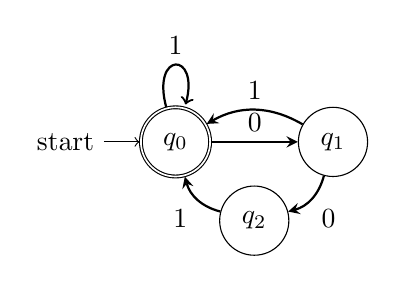
\begin{tikzpicture}[node distance = 2cm]
                \node (q0) [state,initial,accepting] {$q_0$};
                \node (q1) [state] at (2,0) {$q_1$};
                \node (q2) [state] at (1,-1) {$q_2$};

                \path [-stealth, thick]
                    (q0) edge [loop above] node {1} (q0)
                    (q0) edge node [above] {0} (q1)
                    (q1) edge [bend right] node [above] {1} (q0)
                    (q1) edge [bend left] node [below right] {0} (q2)
                    (q2) edge [bend left] node [below left] {1} (q0);
            \end{tikzpicture}
        \end{center}
        }
    \end{q}
    \begin{q}{5}
        Tous les mots qui représente un entier pair en binaire.
        \boxans{\(\left(0\mid1\right)^*0\).\newline
        \begin{center}
            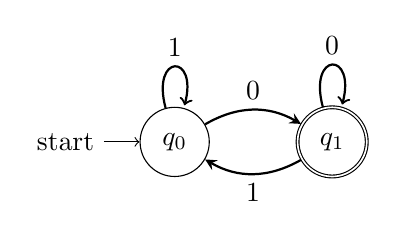
\begin{tikzpicture}[node distance = 2cm]
                \node (q0) [state, initial] {$q_0$};
                \node (q1) [state, accepting] at (2,0) {$q_1$};

                \path [-stealth, thick]
                    (q0) edge [loop above] node {1} (q0)
                    (q1) edge [loop above] node {0} (q1)
                    (q0) edge [bend left] node [above] {0}   (q1)
                    (q1) edge [bend left] node [below] {1}   (q0);
            \end{tikzpicture}
        \end{center}}
    \end{q}
    \begin{q}{6(*)}
        Tous les mots ne contenant pas \(010\).
        \boxans{\((1(0|1)\{2\}|0(11|0(0|1)))^*(0|1)\{0,2\}\)}
    \end{q}
\end{exo}

\begin{exo}
    On considère l'expression rationelle \(\mathcal{E}_1=(a|\eps)(b|\eps)ab(a|\eps)
    (b|\eps)\).
    \begin{q}{1}
        Construire un automate qui reconnait le langage dénoté par \(\mathcal{E}_1\).
        \boxans{
            \begin{center}
                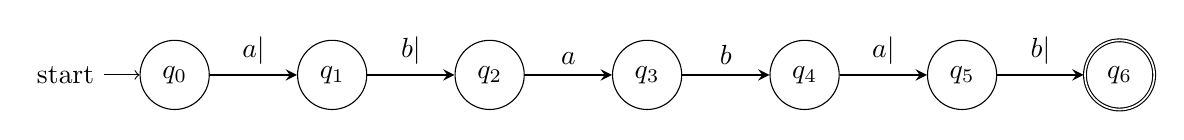
\begin{tikzpicture}[node distance = 2cm]
                    \node (q0) [state, initial] {$q_0$};
                    \node (q1) [state] at (2,0) {$q_1$};
                    \node (q2) [state] at (4,0) {$q_2$};
                    \node (q3) [state] at (6,0) {$q_3$};
                    \node (q4) [state] at (8,0) {$q_4$};
                    \node (q5) [state] at (10,0) {$q_5$};
                    \node (q6) [state,accepting] at (12,0) {$q_6$};

                    \path [-stealth, thick]
                        (q0) edge node [above] {$a|\eps$} (q1)
                        (q1) edge node [above] {$b|\eps$} (q2)
                        (q2) edge node [above] {$a$} (q3)
                        (q3) edge node [above] {$b$} (q4)
                        (q4) edge node [above] {$a|\eps$} (q5)
                        (q5) edge node [above] {$b|\eps$} (q6);
                \end{tikzpicture}
            \end{center}
        }
    \end{q}
    \begin{q}{2}
        Déterminisez l'automate et éliminez les \(\eps\)-transitions.
        \boxans{
            \begin{center}
                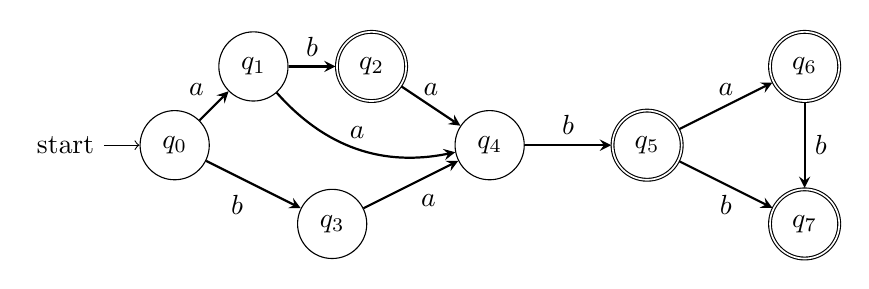
\begin{tikzpicture}[node distance = 2cm]
                    \node (q0) [state, initial] {$q_0$};
                    \node (q1) [state] at (1,1) {$q_1$};
                    \node (q2) [state, accepting] at (2.5,1) {$q_2$};
                    \node (q3) [state] at (2,-1) {$q_3$};
                    \node (q4) [state] at (4,0) {$q_4$};
                    \node (q5) [state, accepting] at (6,0) {$q_5$};
                    \node (q6) [state, accepting] at (8,1) {$q_6$};
                    \node (q7) [state, accepting] at (8,-1) {$q_7$};

                    \path [-stealth, thick]
                        (q0) edge node [above left] {$a$} (q1)
                        (q1) edge node [above] {$b$} (q2)
                        (q0) edge node [below left] {$b$} (q3)
                        (q2) edge node [above] {$a$} (q4)
                        (q3) edge node [below right] {$a$} (q4)
                        (q1) edge [bend right] node [above] {$a$} (q4)
                        (q4) edge node [above] {$b$} (q5)
                        (q5) edge node [above] {$a$} (q6)
                        (q5) edge node [below] {$b$} (q7)
                        (q6) edge node [right] {$b$} (q7);
                \end{tikzpicture}
            \end{center}
        }
    \end{q}
    \begin{q}{3(*)}
        Donner un automate déterministe correspondant à \(\mathcal{E}_2=(a|ba)^*(b|ba)\).
        \boxans{
            \begin{center}
                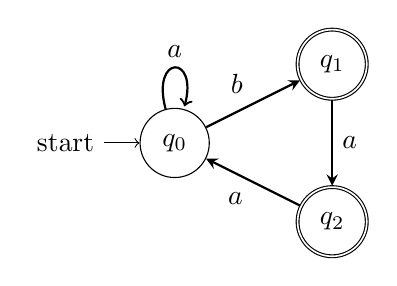
\begin{tikzpicture}
                    \node (q0) [state, initial] {$q_0$};
                    \node (q1) [state, accepting] at (2,1) {$q_1$};
                    \node (q2) [state, accepting] at (2,-1) {$q_2$};

                    \path [-stealth, thick]
                        (q0) edge [loop above] node {$a$} (q0)
                        (q0) edge node [above left] {$b$} (q1)
                        (q1) edge node [right] {$a$} (q2)
                        (q2) edge node [below left] {$a$} (q0);
                \end{tikzpicture}
            \end{center}
        }
    \end{q}
\end{exo}

\begin{exo}
    On considère maintenant l'alphaber ASCII entier. Écrire des regex reconnaissant
    les langages suivants :
    \begin{q}{1}
        Les adresses mail du type \textit{<prenom>.<nom>@u-paris.fr}.
        \boxans{\textbf{(?<prenom>\(\backslash\)w+)\(\backslash\).(?<nom>\(\backslash\)
        w+)@u-paris\(\backslash\).fr}}
        % ^(?<prenom>\w+)\.(?<nom>\w+)@u-paris\.fr$
    \end{q}
    \begin{q}{2}
        Accepter aussi les adresses en \textit{@etu.u-paris.fr}.
        \boxans{\textbf{(?<prenom>\(\backslash\)w+)\(\backslash\).(?<nom>\(\backslash\)
        w+)@(?:etu\(\backslash\).)?u-paris\(\backslash\).fr}}
        % ^(?<prenom>\w+)\.(?<nom>\w+)@(?:etu\.)?u-paris\.fr$
    \end{q}
    \begin{q}{3}
        Les noms de variables dans la majorité des langages, peuvent contenir chiffres,
        lettres, underscores mais doit commencer par une lettre.
        \boxans{\textbf{[a-z,A-Z][a-z,A-Z,0-9,\_]*}}
    \end{q}
\end{exo}

\begin{exo}
    Pour chacun des langages suivant, dire s'il est rationel ou pas.
    \begin{q}{1}
        \(\{a^mb^n\mid m,n\in\N\}\)
        \boxans{Ce langage est reconnu par l'expression : \(a^*b^*\).
        Il est donc rationnel.}
    \end{q}
    \begin{q}{2}
        \(\{a^nb^n\mid n\in\N\}\)
        \boxans{Supposons par l'absurde que le langage est rationel, notons \(N\) l'entier
        donné par le lemme de l'étoile, on considère le mot \(m=a^Nb^N\) qui est dans le
        langage. Aussi les \(x\) et \(y\) du lemme de l'étoile ne peuvent contenir que
        des \(a\) donc le mot \(xy^2z\) contient plus de \(a\) que de \(b\) et n'est donc
        pas dans le langage, qui n'est donc pas régulier.}
    \end{q}
    \begin{q}{3}
        \(\{a^nb^nc^n\mid n\leq 2024\}\)
        \boxans{Ce langage est fini, il est donc rationnel.}
    \end{q}
    \begin{q}{4}
        \(\{u^2\mid u\in \{a,b\}\}\)
        \boxans{Supposons par l'absurde que le langage est rationel, notons \(N\) l'entier
        donné par le lemme de l'étoile, on considère le mot \(u=ab^N\) alors le mot \(m\)
        et de la forme \(ab\dots bab\dots b\). Si \(y\) contient la lettre \(a\) alors avec
        \(k=0\) on a un nombre impair de \(a\) donc un mot qui n'est pas dans le langage.
        Sinon \(y\) contient au moins un \(b\) et donc selon la valeur de \(k\) on fait
        varier la longueur du premier bloc de \(b\) sans changer le second, on obtient
        des mots hors du langage, c'est absurde.}
    \end{q}
    \begin{q}{5}
        \(\{a^mb^n\mid m\neq n\}\)
        \boxans{Supposons par l'absurde que le langage est rationel, notons \(N\) l'entier
        non nul donné par le lemme de l'étoile, on considère le mot \(u=a^Nb^{N!+N}\) qui est
        dans le langage. Alors \(x\) et \(y\) ne contiennent que des \(a\) ainsi quelque
        soit la longueur de \(y\) c'est un diviseur de \(N!\) car inférieur à \(N\) ainsi
        pour le bon entier \(k\) on a autant de \(a\) que de \(b\), et donc un mot
        hors du langage, ce qui est absurde.}
    \end{q}
    \begin{q}{6}
        \(\{u\in \{a,b\}^* \mid u \textrm{ est un palindrome}\}\)
    \end{q}
\end{exo}

\end{document}